\chapter{Conclusion}
brief of conclusion

\section{Conclusion of Problems}
Tell about solving the problem

\section{Conclusion of Method}
Tell about solving using method

\section{Conclusion of Experiment}
Tell about solving in the experiment

\section{Conclusion of Result}
tell about result for purpose of this research.

\section{Andi Muh Aslam/1164064}
\subsection{Teori}
\begin{enumerate}
\item Jelaskan Kenapa Kata-Kata harus dilakukan vektorisasi lengkapi dengan ilustrasi gambar.
\subitem Kata-kata harus dilakukan vektorisasi untuk mengukur nilai kemunculan suatu kata agar dapat di prediksi atau untuk menentukan bobot suatu kata.
\par Untuk ilustrasinya dapat dilihat pada gambar
\begin{figure}[ht]
	\centerline{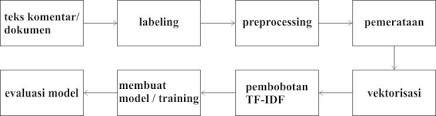
\includegraphics[width=1\textwidth]{figures/andi/L1.PNG}}
	\caption{Ilustrasi Soal No.1}
\end{figure}

\item Jelaskan Mengapa dimensi dari vektor dataset google bisa mencapai 300 lengkapi dengan ilustrasi gambar.
\subitem Dimensi dari vektor dataset google dapat mencapai 300 karena dimensi pada vektor agar dapat membandingkan bobot dari kata tersebut, misalkan terdapat kata Jaket dan Tas pada data set google setiap kata tersebut di buat dimensi vektor senilai 300 kata Jaket dan 300 kata Tas, agar dapat membandingkan bobot dari kesamaan kata Jaket dan Tas. 
\par Untuk ilustrasinya dapat dilihat pada gambar 
\begin{figure}[ht]
	\centerline{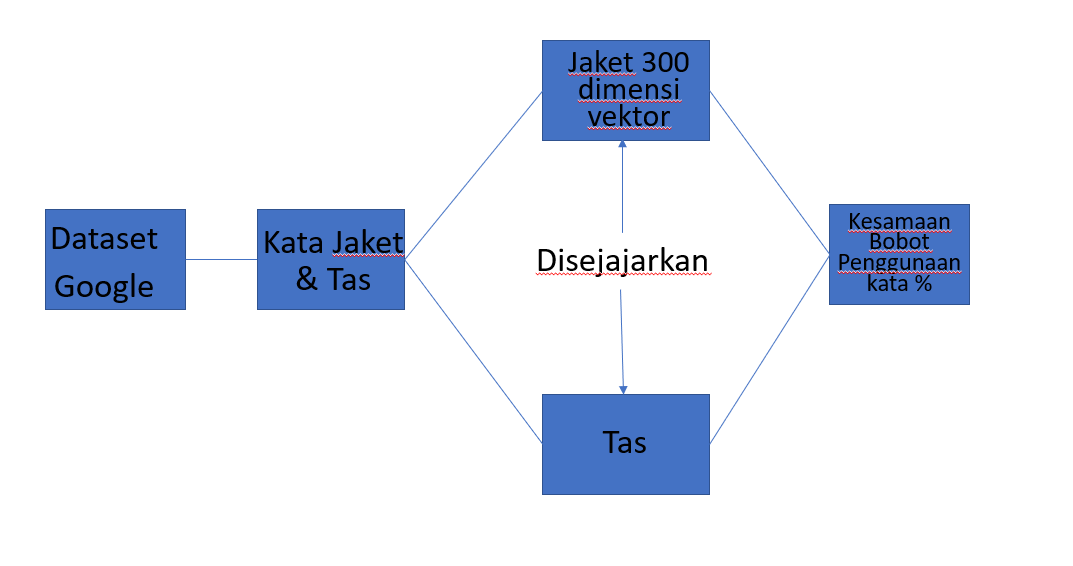
\includegraphics[width=1\textwidth]{figures/andi/L2.PNG}}
	\caption{Ilustrasi Soal No. 2}
	
\end{figure}

\item Jelaskan Konsep vektorisasi untuk kata . dilengkapi dengan ilustrasi atau gambar.
\subitem Konsep dari vektorisasi kata yaitu agar dapat mengetahui kata tengah pada kalimat utama, Contoh ( Subscribe channel ini dan Like yah Guys ). Kata tengah dari contoh tersebut merupakan (dan) yang memiliki bobot sebagai kata tengah dari kalimat. Hal ini sangat berkaitan dengan dimensi vektor pada dataset google karena memiliki nilai atau bobot kata tengah.
\par Untuk ilustrasinya dapat dilihat pada gambar \begin{figure}[ht]
	\centerline{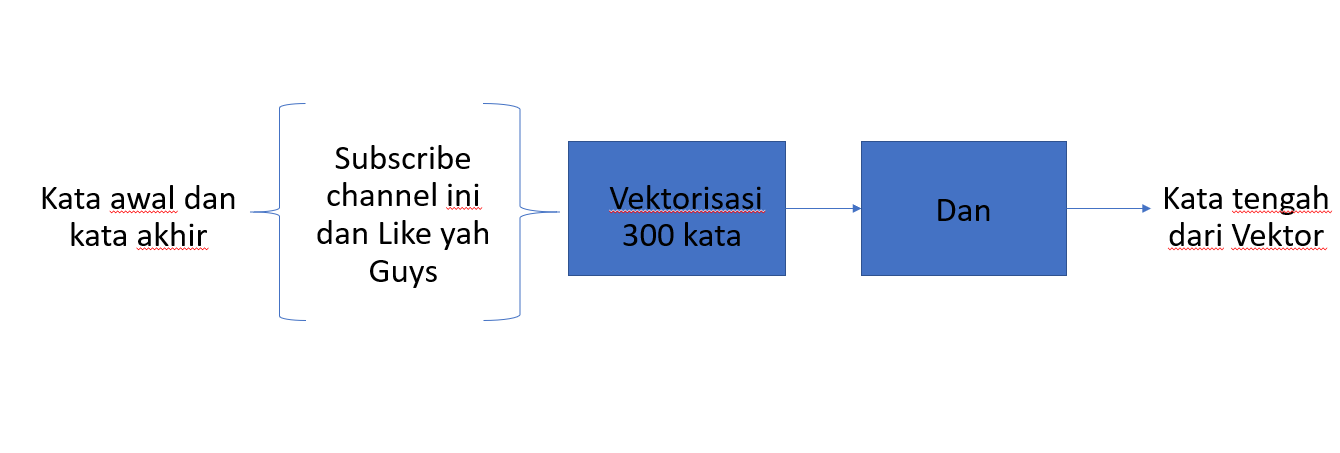
\includegraphics[width=1\textwidth]{figures/andi/L3.PNG}}
	\caption{Ilustrasi Soal No. 3}
	
\end{figure}
\item Jelaskan Konsep vektorisasi untuk dokumen. dilengkapi dengan ilustrasi atau gambar.
\subitem Konsep vektorisasi pada dokumen mesin akan membaca kata-kata terlebih dahulu pada semua kalimat yang ada di dalam dokumen dan nanti kalimat yg ada di dalam dokumen akan dipecah menjadi kata-kata.
\par Untuk ilustrasinya dapat dilihat pada gambar 
\begin{figure}[ht]
	\centerline{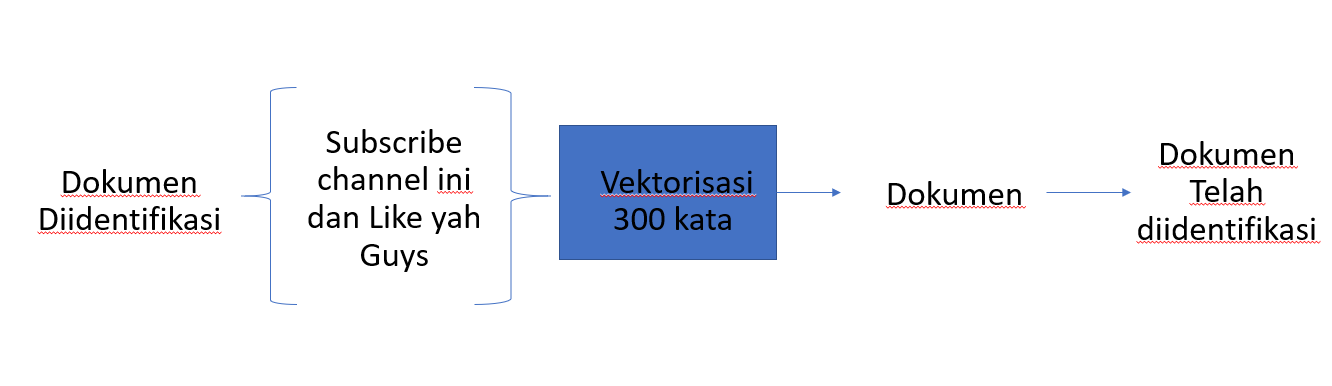
\includegraphics[width=1\textwidth]{figures/andi/L4.PNG}}
	\caption{Ilustrasi Soal No. 4}
	
\end{figure}

\item Jelaskan apa mean dan standar deviasi, lengkapi dengan iludtrasi atau gambar.
\subitem Mean merupakan nilai rata-rata yang tingkat akurasinya tinggi atau nilai tersebut sering munucul. Standar deviasi mengukur bagaimana nilai-nilai data tersebar. Bisa juga didefinisikan sebagai, rata-rata jarak penyimpangan titik-titik data diukur dari nilai rata-rata data tersebut.
\par Untuk ilustrasinya dapat dilihat pada gambar 
\begin{figure}[ht]
	\centerline{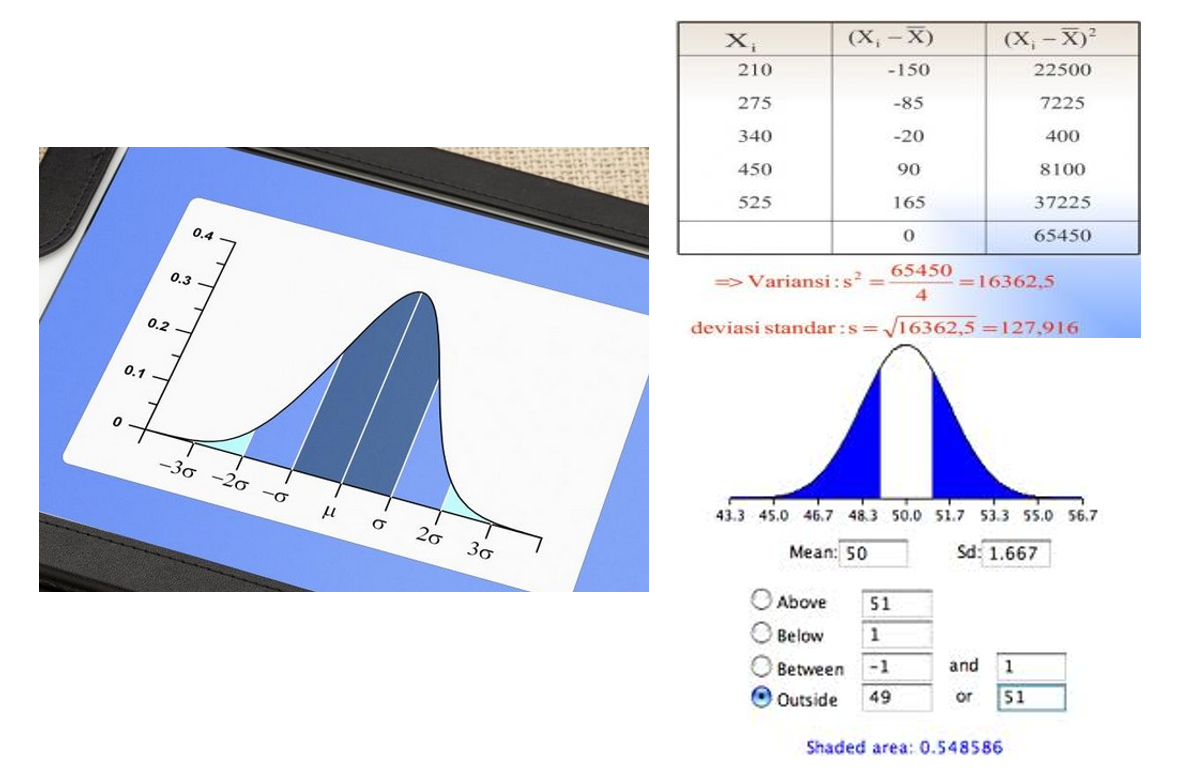
\includegraphics[width=1\textwidth]{figures/andi/L5.PNG}}
	\caption{Ilustrasi Soal No. 5}
	
\end{figure}

\item Jelaskan Apa itu Skip-Gram sertakan contoh ilustrasi.
\subitem Skip-Gram yaitu dimana kata tengah menjadi acuan terhadap kata kata pelengkap dalam suatu kalimat.
\par Untuk ilustrasinya dapat dilihat pada gambar 
\begin{figure}[ht]
	\centerline{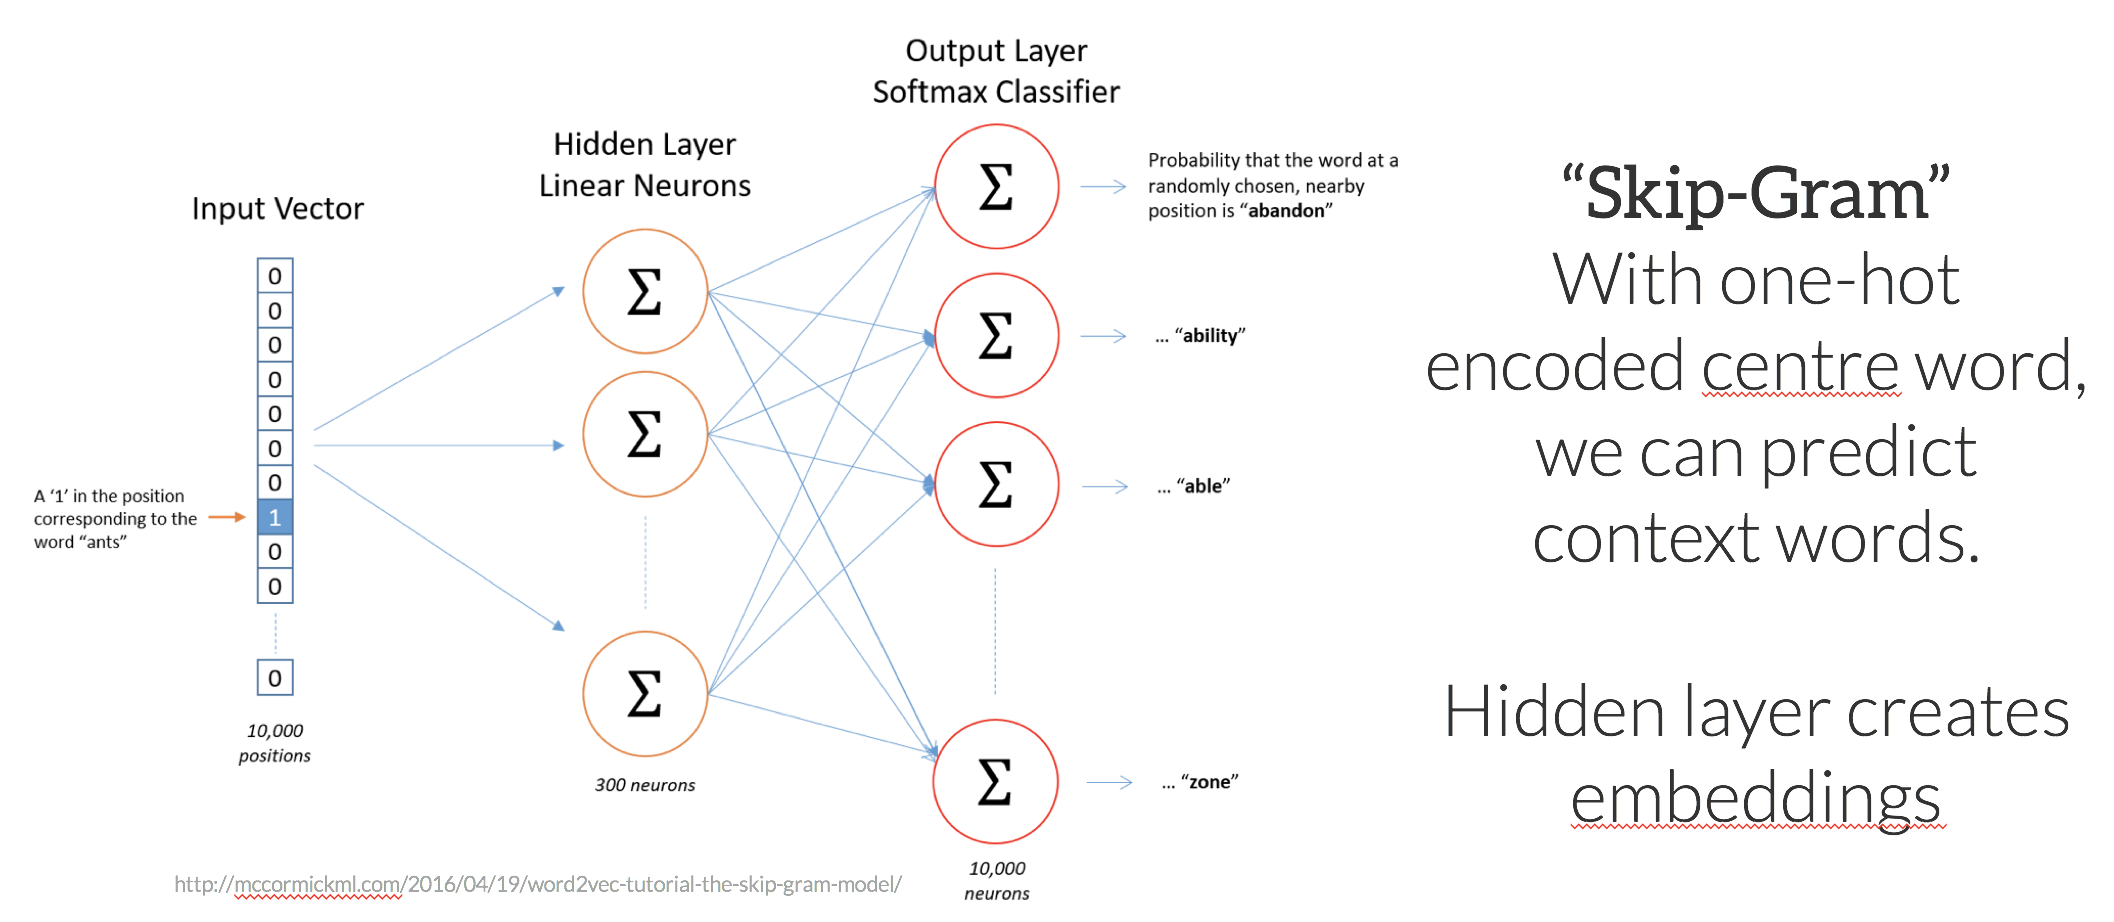
\includegraphics[width=1\textwidth]{figures/andi/L6.PNG}}
	\caption{Ilustrasi Soal No. 6}
	
\end{figure}
\end{enumerate}

